%corpus--语料库
\section{语料库}
自然语言处理显然少不了使用语料库,这里使用的语料库有kiki简体中文语料,复旦大学,搜狗.下面重点介绍一下这三个语料库的获取和预处理.
\subsection{wiki简体中文语料}
\subsubsection{获取}
wiki语料获取非常方便,链接是\url{http://download.wikipedia.com/zhwiki/},在该目录下面(见图\ref{fig:corpus:wiki})可以找到wiki近期所有的中文语料库,我们使用的20141105目录下面的$zhwiki-20141105-pages-articles-multistream.xml.bz2$文件,这个压缩包有1.1G,里面存放的是标题和正文部分,如果需要其他数据,如页面跳转或历史编辑记录等,可以在当前页面上找对应的链接.
\begin{figure}[!htbp]
	\centering
	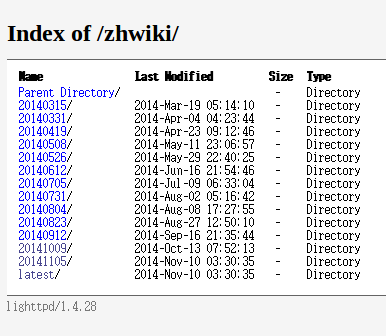
\includegraphics[scale=0.5]{figs/corpus_wiki.png} 
	\caption{wiki下载目录}    
	\label{fig:corpus:wiki}
\end{figure}

\subsubsection{预处理}
对wiki中文语料库的预处理有两步.
\begin{enumerate}
\item 抽取正文文本\\
\begin{lstlisting}[style=BASH]
hjy@hjy:yourworkspace$ bzcat zhwiki-latest-pages-articles.xml.bz2 | python WikiExtractor.py -b1000M -o extracted >output.txt
\end{lstlisting}
上面命令中$bzcat$是将.bz2文件中的.xml文件解压并将里面文本显示到终端,这里用管道$|$将该文本作为下个python程序的输入.$-b1000m$表示以1000M为单位切分文件,默认是500K,由于最后生成的正文文本不到 600M,把参数设置的大一些可以保证最后的抽取结果全部存在一个文件里。执行命令后,获得两个文件,一个是$extracted/AA$目录下的$wiki\_00$文件,里面的文本格式如下
\begin{lstlisting}[style=XML]
<doc id="*" url="*" title="TITLE">
TITLE

TEXT
</doc>
\end{lstlisting}
另一个是$output.txt$,它是对$wiki\_00$中所有的id和title进行了提取.每一对占一行.


\item 繁简转换\\
wiki中文语料库中是简繁混杂的,里面包含大陆简体、台湾繁体、港澳繁体等多种不同的数据。这里使用开源项目opencc进行处理.其在ubuntu上的安装使用如下命令.
\begin{lstlisting}[style=BASH]
hjy@hjy:yourworkspace$ sudo apt-get install opencc
\end{lstlisting}
接着就可以使用该命令对$wiki\_00$和$output.txt$进行繁简转换.
\begin{lstlisting}[style=BASH]
hjy@hjy:yourworkspace$ opencc -i wiki_00 -o wiki_chs -c zht2zhs.ini
\end{lstlisting}
最终我们获得$wiki\_chs$和$wiki\_output\_chs.txt$两个文件.
\end{enumerate}

\subsubsection{优点}
优点有如下三点:
\begin{enumerate}
\item 资源获取非常方便.相比之下,其他很多语料都需要用爬虫抓取,或者付费获得。
\item 文档解析有非常多的成熟工具,直接使用开源工具即可完成正文的提取。
\item 维基百科的质量较高,而且领域广泛
\end{enumerate}

\subsection{复旦语料库}
复旦语料库的下载地址\url{http://www.nlpir.org/?action-viewnews-itemid-103}


\subsection{搜狗语料库精简版}
搜狗语料库的下载地址\url{http://www.sogou.com/labs/dl/c.html}

